%- HandOut Flag -----------------------------------------------------------------------------------------
\makeatletter
\@ifundefined{ifHandout}{%
  \expandafter\newif\csname ifHandout\endcsname
}{}
\makeatother

%- D0cum3nt ----------------------------------------------------------------------------------------------
\documentclass[beamer,10pt]{standalone}   
%\documentclass[beamer,10pt,handout]{standalone}  \Handouttrue  

\ifHandout
	\setbeameroption{show notes} %print notes   
\fi

	
%- Packages ----------------------------------------------------------------------------------------------
\usepackage{custom-style}
\usepackage{math}
\usetikzlibrary{positioning}
\usepackage{multicol}


%--Beamer Style-----------------------------------------------------------------------------------------------
\usetheme{toninus}
\usepackage{animate}
\usetikzlibrary{positioning, arrows}
\usetikzlibrary{shapes}

\begin{document}
%------------------------------------------------------------------------------------------------

\subsection{Regular reduction in symplectic geometry}
%------------------------------------------------------------------------------------------------
\begin{frame}{Reminder: momentum maps in symplectic geometry}\label{frame:symplecticmomaps}
	Consider $\theta:G\curvearrowright M$ symplectic,~~ $\underline{\cdot}:\mathfrak{g}\to \mathfrak{X}(M)$ infinitesimal action.
	\vfill

	\begin{columns}[T]
		\setlength{\belowdisplayskip}{5pt}
		\begin{column}{.50\linewidth}
			%
			\centering \it
			\onslide<2->{
				\begin{defblock}[Equivariant moment map]
					Smooth map $$\mu:M\to \mathfrak{g}^\ast$$
					such that:
					\begin{itemize}
						\item[i.] $d\langle \mu,\xi\rangle = -\iota_{\underline{\xi}}\omega$ 
						~\qquad, $\forall \xi \in \mathfrak{g}$
						\item[ii.] $\mu \circ \theta_g = Ad_g^\ast \circ \mu$
						 \qquad\small, $\forall g \in G$
					\end{itemize}
				\end{defblock}
			}
		\end{column}	
		%
		\onslide<2->{\vrule{}}
		%
		\begin{column}{.50\linewidth}
			\onslide<3->{			
				\begin{defblock}[Comoment map]
					Linear map $$\widetilde{\mu}: \mathfrak{g}\to C^\infty(M,\omega)$$
					such that:
					\begin{itemize}
						\item[i.] $d\widetilde{\mu}(\xi) = -\iota_{\underline{\xi}}\omega$ 
						\qquad~\small, $\forall \xi \in \mathfrak{g}$
						\item[ii.] $\widetilde{\mu}([\xi,\eta]) = \lbrace\widetilde{\mu}(\xi),\widetilde{\mu}(\eta)\rbrace$ \small, $\forall \xi,\eta \in \mathfrak{g}$
					\end{itemize}
				\end{defblock}
			}
		\end{column}	
	\end{columns}	
	%
	\pause
	\vspace{1em}
	%
	\begin{columns}[]
		\setlength{\belowdisplayskip}{5pt}
		\begin{column}{.40\linewidth}
			%
			\centering \it
			\onslide<5->{
				\begin{upshotblocktitle}[Duality]
					\begin{displaymath}
						\mu(x) : \mathfrak{\xi} \mapsto \widetilde{\mu}(\xi)\big\vert_x
					\end{displaymath}
					%
					\emph{
					\small
					"duality wrt. the currying operation"					
					}
				\end{upshotblocktitle}
			}
		\end{column}	
		%
		%
		\begin{column}{.60\linewidth}
			\onslide<4->{			
				\begin{upshotblocktitle}[$\widetilde{\mu}$ as a lift]
					\begin{displaymath}
						\begin{tikzcd}[ampersand replacement = \&]
						 \& C^\infty(M,\omega) \ar[d,"\vHam"]
						 \\
						 \mathfrak{g} \ar[ur,dashed,sloped,"\widetilde{\mu}"]\ar[r,"\underline{\cdot}"'] \& \mathfrak{X}(M)
						\end{tikzcd}
					\end{displaymath}
					%
					\emph{
					\small
					"it is a lift (in the Lie category) of the infinitesimal action by the assigment of hamiltonian v.fields."					
					}
				\end{upshotblocktitle}
			}
		\end{column}	
	\end{columns}		
\end{frame}
\note[itemize]{
	\item consider an action preserving the symplectic form.
	\item[-] $\langle \cdot, \cdot \rangle$ is the natural pairing of $\mathfrak{g}$ and $\mathfrak{g}^\ast$.
		\item[-] $\theta_g$ is the diffeomorphism associated to $g\in G$ via $\theta:G\curvearrowright M$
		\item[-] $Ad^\ast_g$ is the coadjoint action $G\curvearrowright \mathfrak{g}^\ast$
	\item The moment map can be reexpressed as a comomentum map.
	\item Observe that ii. on the left always implies ii. on the right. The converse is trure only if $G$ is connected.
	\item $G\curvearrowright M$ is said "Hamiltonian" (see slide \ref{frame:gisthamaction} in appendix) iff $\exists$ comoment map $\widetilde{\mu}$.
	\item \emph{moment map: Describe ${\color{orange}G\curvearrowright M}$ in terms of $\color{blue}C^\infty(M)\to\X(M)$.}
	\begin{center}
	\begin{tikzpicture}[scale=1.5]
		\node[orange] (A) at (0,0) {$\g$};
		\node[gray] (A1) at (0,-.3) {$\xi$};
		\node[blue] (B) at (1,1) {$C^\infty(M)$};
		\node[gray] (B2) at (1.55,1) {$f$};
		\node[orange] (C) at (1,0) {$\X(M)$};
		\node[gray] (C1) at (1,-.3) {$\underline\xi$};
		\node[gray] (C2) at (1.55,0) {$X_f$};

		\path[->,blue,dashed] (A) edge node[above left] {$\langle\mu,\cdot\,\rangle$} (B);
		\path[->,orange] (A) edge (C);
		\path[->] (B) edge (C);
		\path[|->,gray] (A1) edge (C1);
		\path[|->,gray] (B2) edge (C2);

		\begin{scope}[xshift=3cm]
			\node at (-.32,.8) {as Lie algebras};
			\node at (-.13,.2) {i.e., {\color{blue}$\mu_\xi$} generates {\color{orange}$\underline\xi$}};
		\end{scope}
	\end{tikzpicture}
	
		\footnotesize		(\emph{moment map:} ${\color{blue}\mu:M\to\g^*}$, 
	 \emph{Hamiltonian $G$-space:} 	$(M,\omega,G,\mu)$)
	\end{center}
	\item
	 $\alpha\mapsto X_\alpha$ is a homomorphism of Leibniz algebras:
	$$\d\{\alpha,\beta\} = \d\L_{X_\alpha}\beta = \L_{X_\alpha}\iota_{X_\beta}\omega = \iota_{[X_\alpha,X_\beta]}\omega ~{\color{black!80} \implies}~
	X_{\{\alpha,\beta\}} = [X_\alpha,X_\beta]$$
}
%------------------------------------------------------------------------------------------------

%------------------------------------------------------------------------------------------------
\begin{frame}{Reminder: regular reduction in symplectic geometry}
	\textbf{\color{UniGreen}Symplectic reduction:}~~
	\\ 
	{\it \small
	Procedure associating to any (suitably regular) pair of symplectic manifold and Hamiltonian action another symplectic manifold of smaller dimension.}
	\vfill
	\pause
	\begin{thmblock}[Marsden-Weinstein reduction \cite{MarsdenWeinstein74}]
		\vspace{-.4em}\hspace{-1em}
		\begin{tabular}{l p{14cm}}
		    Given: & $(M,\omega)$ symplectic
		    \\
		    & $G\curvearrowright M$ symplectic with equivariant momap. $\mu:M\to \mathfrak{g}^*$
		    \\[.2em]
		    Assume: & $\phi \in \mathfrak{g}^*$ regular value of $\mu$ 
		    \qquad\quad \footnotesize \textcolor{gray}{($\Rightarrow$ $\mu^{-1}(\phi)\hookrightarrow M$ smooth embedding)}
		    \\
			& $G_\phi\curvearrowright \mu^{-1}(\phi)$ free and proper
			\quad \footnotesize \textcolor{gray}{($\Rightarrow$ $\mu^{-1}(\phi)/G_\phi$ smooth manifold)}
			\\[.4em]
			Then: & $\exists!$ symplectic structure $\omega_\phi$ in $M_\phi:= \mu^{-1}(\phi)/G_\phi$ \\
			& s.t. $\pi^\ast \omega_\phi = j^\ast \omega$ 
			\qquad {\footnotesize with $j:\mu^{-1}(\phi) \hookrightarrow M$ and $\pi:\mu^{-1}(\phi)\twoheadrightarrow M_\mu$}
		\end{tabular}
		\vspace{-.4em}
	\end{thmblock}
	%
	\vfill
	\pause
	\begin{columns}
		\begin{column}{0.40\textwidth}
			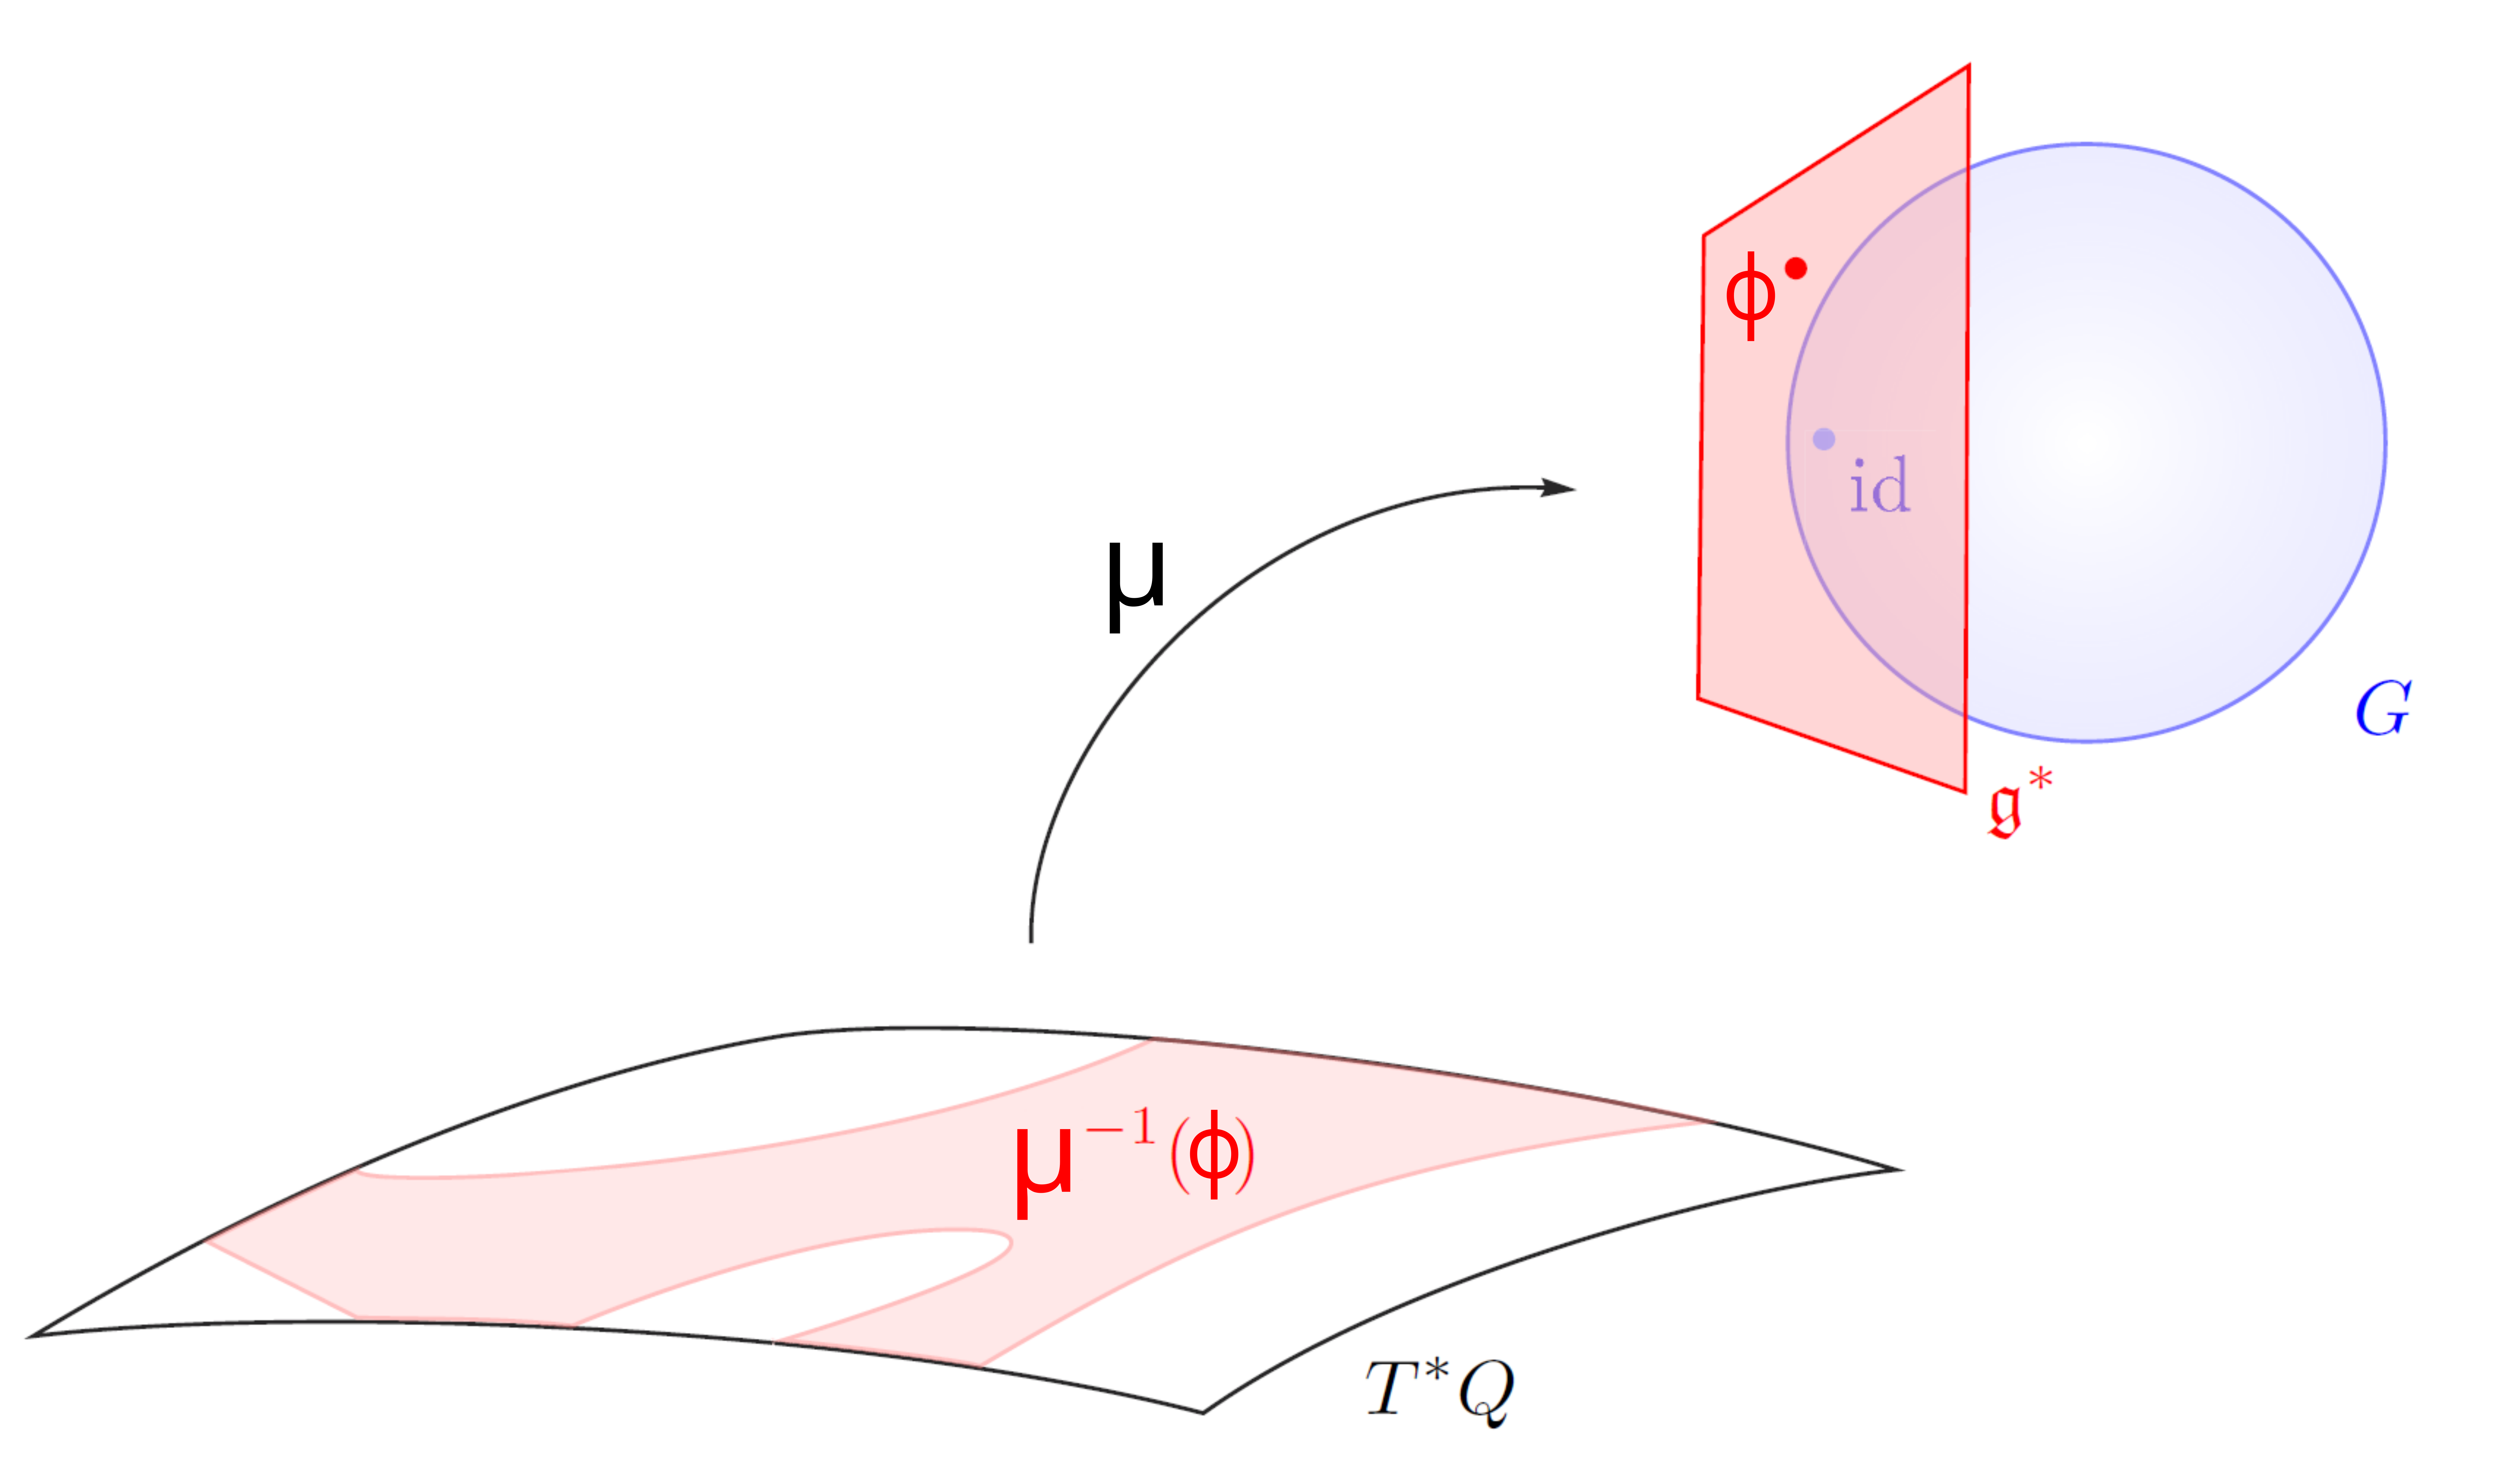
\includegraphics[width=\textwidth]{Pictures/Reduction}
		\end{column}	
		
		\begin{column}{0.6\textwidth}
				\textbf{\color{UniGreen}In mechanics:}~~
				\\
			{\it \small
				it embodies the process of restricting the dynamics of the system to the level sets of the conserved quantities pertaining to the symmetry group.		
			}
			\\[.2em]
			\color{gray}\small( e.g. restricting to studying a point-like particle in a central potential by studying it in radial coordinates)
		\end{column}	
	\end{columns}	
\end{frame}
\note[itemize]{
	\item {Symplectic Reduction} takes two inputs:
	\\ 1. Hamiltonian $G$-space $(M,\omega,{\color{orange}G},{\color{blue}\mu})$
	\\ 2. parameter ${\color{blue}\phi}\in\g^*$
	\item The \emph{reduced space} is $M_\phi:={\color{blue}\mu^{-1}(\phi)}{\color{orange}/G_\phi}$.
	\item (Marsden--Weinstein '74, Meyer '73) THM:\\
		If $\mu^{-1}(\phi)\subset M$ is smooth and $G_\phi\curvearrowright \mu^{-1}(\phi)$ is free and proper, then there is a \textbf{unique symplectic form} $\omega_\phi\in\Omega^2(M_\phi)$ such that $\pi^*\omega_\phi = i^*\omega$.


	\begin{center}
	\begin{tikzpicture}[scale=2]
		\node[blue] (A) at (0,0) {$\mu^{-1}(\phi)$};
		\node[gray] (A1) at (0,.3) {$i^*\omega$};
		\node[gray] (A2) at (-.6,0) {$\pi^*\omega_\phi$};
		\node[blue] (B) at (1,0) {$M$};
		\node[gray] (B1) at (1,.3) {$\omega$};
		\node[orange] (C) at (0,-.8) {$M_\phi$};
		\node[gray] (C2) at (-.6,-.8) {$\omega_\phi$};

		\path[right hook->,blue] (A) edge node[above] {$i$} (B);
		\path[orange,->] (A) edge node[left] {$\pi$} (C);

		\begin{scope}[xshift=-1.8cm]
			\node[blue] at (0,0) {\small restrict to $\{\mu=\phi\}$};
			\node[orange] at (.15,-.4) {\small quotient by $G_\phi$};
		\end{scope}
	\end{tikzpicture}
	\end{center}
	\item Heuristic Approach to Reduction:
	\\1. describe $G\curvearrowright M$ in terms of $\omega$ 	\hspace{1cm}
	({\color{green}moment map $\mu$})
	\\2. identify a distinguished reduced space \hspace{1cm}
	({\color{green}reduction at $\mu=0$})
	\\3. use the ambiguity in 1.\ to obtain a family of reduced spaces \hspace{1cm}
	({\color{green}reduction at $\mu-\phi=0$, i.e.\ reduction at $\mu=\phi$}
	\\
	{\tiny Note: If $G_\phi\neq G$, then $\mu-\phi:M\to\g^*$ is not a moment map for either $G\curvearrowright M$ or $G_\phi\curvearrowright M$.}
	
}
%------------------------------------------------------------------------------------------------

\subsection{Regular reduction in multisymplectic geometry}
%------------------------------------------------------------------------------------------------
\begin{frame}{Momentum maps in multisymplectic geometry}
	Consider $\theta:G\curvearrowright M$ {\color{UniGreen}multi}symplectic,~~ $\underline{\cdot}:\mathfrak{g}\to \mathfrak{X}(M)$ infinitesimal action.
	\vfill

	\begin{columns}[T]
		\setlength{\belowdisplayskip}{5pt}
		\begin{column}{.50\linewidth}
			%
			\centering \it
			\onslide<2->{
				\begin{defblock}[Equivariant moment map]
					Smooth map $$\mu:M\to \mathfrak{g}^\ast{\color{UniGreen}\otimes \Lambda^{n-1}T^\ast M}$$
					such that:
					\begin{itemize}
						\item[i.] $d\langle \mu,\xi\rangle = -\iota_{\underline{\xi}}\omega$ \qquad\qquad \small,$\forall \xi \in \mathfrak{g}$
						\item[ii.] $\mu \circ \theta_g = \left(Ad_g^\ast {\color{UniGreen} \,\otimes\, \theta^\ast_g}\right) \circ \mu$ \quad \small, $\forall g \in G$
						\item[iii.] {\color{UniGreen} $\mu \in \Omega^{n-1}(M,\mathfrak{g}^\ast)$}
					\end{itemize}
				\end{defblock}
			}
		\end{column}	
		%
		\onslide<2->{\vrule{}}
		%
		\begin{column}{.50\linewidth}
			\onslide<3->{			
				\begin{defblock}[Comoment map]
					Linear map $$\widetilde{\mu}: \mathfrak{g}\to {\color{UniGreen}Leib(M,\omega)}$$
					such that:
					\begin{itemize}
						\item[i.] $d\widetilde{\mu}(\xi) = -\iota_{\underline{\xi}}\omega$ 
						\qquad~\small, $\forall \xi \in \mathfrak{g}$
						\item[ii.] $\widetilde{\mu}([\xi,\eta]) = {\color{UniGreen}\llbracket \widetilde{\mu}(\xi),\widetilde{\mu}(\eta)\rrbracket}$ \small, $\forall \xi,\eta \in \mathfrak{g}$
					\end{itemize}
				\end{defblock}
			}
		\end{column}	
	\end{columns}	
	%
	\pause
	\vfill
	%
	\begin{columns}[]
		\setlength{\belowdisplayskip}{5pt}
		\begin{column}{.40\linewidth}
			%
			\centering \it
			\onslide<5->{
				\begin{upshotblocktitle}[Duality]
					\begin{displaymath}
						\mu(x) : \mathfrak{\xi} \mapsto \widetilde{\mu}(\xi)\big\vert_x
					\end{displaymath}
					%
					\emph{
					\small
					"duality wrt. the currying operation"					
					}
				\end{upshotblocktitle}
			}
		\end{column}	
		%
		%
		\begin{column}{.60\linewidth}
			\onslide<4->{			
				\begin{upshotblocktitle}[$\widetilde{\mu}$ as a lift]
					\begin{displaymath}
						\begin{tikzcd}[ampersand replacement = \&]
						 \& {\color{UniGreen}Leib(M,\omega)} \ar[d,"\vHam"]
						 \\
						 \mathfrak{g} \ar[ur,dashed,sloped,"\widetilde{\mu}"]\ar[r,"\underline{\cdot}"'] \& \mathfrak{X}(M)
						\end{tikzcd}
					\end{displaymath}
					%
					\emph{
					\small
					"it is a lift (in the {\color{UniGreen}Leibniz} category) of the infinitesimal action by the assigment of hamiltonian v.fields."					
					}
				\end{upshotblocktitle}
			}
		\end{column}	
	\end{columns}		
\end{frame}
\note[itemize]{
	\item consider an action preserving the multisymplectic form.
		\item[-] $\langle \cdot, \cdot \rangle$ is the natural pairing of $\mathfrak{g}$ and $\mathfrak{g}^\ast$.
		\item[-] $\theta_g$ is the diffeomorphism associated to $g\in G$ via $\theta:G\curvearrowright M$
		\item[-] $Ad^\ast_g$ is the coadjoint action $G\curvearrowright \mathfrak{g}^\ast$
		\item[-] $\theta^\ast_g$ is the induced action $G\curvearrowright \Lambda^{n-1}T^\ast M$ (lift on differential forms)		
	\item As before, The moment map can be reexpressed as a comomentum map. 
	\item As before that ii. on the left always implies ii. on the right. The converse is trure only if $G$ is connected.
	\item \emph{moment map: Describe ${\color{orange}G\curvearrowright M}$ in terms of
			$\underset{{\color{blue}\Omega_H^{k-1}(M)}}{\text{\cancel{${\color{blue}C^\infty(M)}$}}} \;{\color{blue}\to\X(M)}$.}

	\begin{center}
	\begin{tikzpicture}[scale=1.5]
		\node[orange] (A) at (0,0) {$\g$};
		\node[gray] (A1) at (0,-.3) {$\xi$};
	\node[blue] (B) at (1,1) {$\Omega_H^{k-1}(M)$};
		\node[gray] (B2) at (1.55,1) {$\alpha$};
		\node[orange] (C) at (1,0) {$\X(M)$};
		\node[gray] (C1) at (1,-.3) {$\underline\xi$};
		\node[gray] (C2) at (1.55,0) {$X_\alpha$};

		\path[->,blue,dashed] (A) edge node[above left] {$\langle\mu,\cdot\,\rangle$} (B);
		\path[->,orange] (A) edge (C);
		\path[->] (B) edge (C);
		\path[|->,gray] (A1) edge (C1);
		\path[|->,gray] (B2) edge (C2);

		\begin{scope}[xshift=3cm]
			\node at (.07,.8) {as Leibniz algebras \phantom{\color{black!50}($\pm1$)}};
			\node at (-.13,.2) {i.e., {\color{blue}$\mu_\xi$} generates {\color{orange}$\underline\xi$}};
			%\node at (-.39,.2) {{\color{black!50}i.e.} $X_{\color{blue}\mu_\xi} = {\color{orange}\underline\xi}$};
		\end{scope}
	\end{tikzpicture}

	\footnotesize		(
		\emph{moment map:}		${\color{blue}\mu\in\Omega^{k-1}(M,\g^*)}$	
		\emph{Hamiltonian $G$-space:}	$(M,\omega,G,\mu)$)	
	\end{center}
}
%------------------------------------------------------------------------------------------------

%------------------------------------------------------------------------------------------------
\begin{frame}{Regular reduction in multisymplectic geometry}
	Let $(M,\omega)$ be $n$-plectic.
	Consider an action $G\curvearrowright M$ with moment map $\mu$.

	\pause
	\vfill
	\begin{defblock}[Regular value of $\mu$]
		Closed differential form $\phi \in \Omega^{n-1}(M,\mathfrak{g}^\ast)$, such that
		$$
		 \mu^{-1}(\phi)=\lbrace x \in M ~ \vert ~ \mu(x)=\phi(x)\rbrace
		$$
		is a smoothly embedded into $M$.	
	\end{defblock}	
	
	\pause
	\vfill
	

	\begin{thmblock}[Multisymplectic regular reduction \cite{Blacker20}]
		\vspace{-.4em}\hspace{-1em}
		\begin{tabular}{l p{14cm}}
		    Given: & $(M,\omega)$ {\color{UniGreen}$n$-}plectic
		    \\
		    & $G\curvearrowright M$ {\color{UniGreen}multi}symplectic with equivariant momap. {\color{UniGreen}$\mu\in \Omega^{n-1}(M,\mathfrak{g}^*)$}
		    \\[.2em]
		    Assume: & $\phi \in {\color{UniGreen} \Omega^{n-1}(M,\mathfrak{g}^*)}$ regular value of $\mu$ 
		    \quad\quad \footnotesize \textcolor{gray}{($\mu^{-1}(\phi)\hookrightarrow M$ embedding)}
		    \\
			& $G_\phi\curvearrowright \mu^{-1}(\phi)$ free and proper
			\quad\qquad \footnotesize \textcolor{gray}{($\mu^{-1}(\phi)/G_\phi$ smooth manifold)}
			\\[.4em]
			Then: & $\exists!$ {\color{UniGreen}pre-n-}plectic structure $\omega_\phi$ in $M_\phi:= \mu^{-1}(\phi)/G_\phi$ \\
			& s.t. $\pi^\ast \omega_\phi = j^\ast \omega$ 
			\qquad {\footnotesize with $j:\mu^{-1}(\phi) \hookrightarrow M$ and $\pi:\mu^{-1}(\phi)\twoheadrightarrow M_\mu$}
		\end{tabular}
		\vspace{-.4em}
	\end{thmblock}	
	
\end{frame}
\note[itemize]{
	\item First: introduce the higher analague of a "regular value" for the higher comomentum map.
	\item The notion of $G$-equivariant covariant moment map turns out to be the right prerequisite for reduction in the multisymplectic setting. Somewhat surprisingly, this is true, even for the ($L_\infty$-)algebraic reduction, where one might expect homotopy moment maps, which directly interact with the involved $L_\infty$-structures to play a role.
	\item pre-$n$-plectic means closed and possibly degenerate.
	\item {Multisymplectic Reduction} takes Two inputs:
	\\1. Hamiltonian $G$-space $(M,\omega,{\color{orange}G},{\color{blue}\mu})$
	\\2. parameter ${\color{blue}\phi}\in\Omega^{k-1}(M,\g^*)$ with $\d\phi=0$
	\item 
	The \emph{reduced space} is $M_\phi:={\color{blue}\mu^{-1}(\phi)}{\color{orange}/G_\phi}$
	\item THM:
		If $\mu^{-1}(\phi)\subset M$ is smooth and $G_\phi\curvearrowright\mu^{-1}(\phi)$ is free and proper, then there is a \textbf{unique closed $(k+1)$-form} $\omega_\phi$ on $M_\phi$ such that $\pi^*\omega_\phi = i^*\omega$.
	\begin{center}
	\begin{tikzpicture}[scale=1.5]
		\node[blue] (A) at (0,0) {$\mu^{-1}(\phi)$};
		\node[gray] (A1) at (0,.3) {$i^*\omega$};
		\node[gray] (A2) at (-.6,0) {$\pi^*\omega_\phi$};
		\node[blue] (B) at (1,0) {$M$};
		\node[gray] (B1) at (1,.3) {$\omega$};
		\node[orange] (C) at (0,-.8) {$M_\phi$};
		\node[gray] (C2) at (-.6,-.8) {$\omega_\phi$};

		\path[right hook->,blue] (A) edge node[above] {$i$} (B);
		\path[->,orange] (A) edge node[left] {$\pi$} (C);

		\begin{scope}[xshift=-2cm]
			\node[blue] at (0,0) {\small restrict to $\{\mu=\phi\}$};
			\node[orange] at (.15,-.6) {\small quotient by $G_\phi$};
		\end{scope}
	\end{tikzpicture}
	\end{center}
	
}
%------------------------------------------------------------------------------------------------

\end{document}